\documentclass{report}

\usepackage[T2A]{fontenc}
\usepackage[utf8]{inputenc}
\usepackage[english, russian]{babel}

\usepackage[letterpaper,top=2cm,bottom=2cm,left=3cm,right=3cm,marginparwidth=1.75cm]{geometry}

\usepackage{amsmath}
\usepackage{graphicx}
\usepackage[colorlinks=true, allcolors=blue]{hyperref}
\usepackage{listings}

\begin{document}

\newpage
\chapter{Обработка исключительных ситуаций}

\section{Концепция обработки исключений}

\textbf{Исключительная ситуация} – это программная ошибка, которая возникает во время выполнения последовательности программного кода. Программная ошибка может быть логической ошибкой программиста во время разработки программы. Например, исключительная ситуация может возникать в случаях:

\begin{enumerate}
    \item попытки деления на нуль;
    \item попытки обращения к элементу массива, номер индекса которого выходит за пределы объявленного;
    \item попытки взять корень из отрицательного числа;
    \item попытки открыть файл по имени, которого нет на диске;
    \item другие случаи.
\end{enumerate}

Как правило, каждая исключительная ситуация может иметь свой код ошибки и обработку этого кода (вывод соответствующих сообщений, и т.п.). В языке программирования Java разработан механизм обработки исключительных ситуаций.

В языке программирования Java, \textbf{исключение} – это специальный объект, описывающий исключительную ситуацию, которая возникла в некоторой части программного кода. Объект представляющий исключение, генерируется в момент возникновения исключительной ситуации. После возникновения критической (исключительной) ситуации исключение перехватывается и обрабатывается. Таким образом, возникает понятие \textbf{ генерирования исключения}. Генерирование исключения – процесс создания объекта, который описывает данное исключение.

Исключения могут генерироваться либо автоматически — через исполняемую систему Java, при нарушении ограничений системы языка, — либо вручную — через программный код. Первый случай происходит, если в самом коде нету \textbf{блока обработки и перехвата} исключений или же он имеется, но не обрабатывает данное исключение.

Обычно для блока исключений используются следующие ключевые слова:

\begin{enumerate}
    \item \verb|try| — указывает начало блока кода, в котором возможно исключение(я);
    \item \verb|catch| — указывает начало блока кода, который запускается при срабатывании определённого типа исключения;
    \item \verb|throw| — используется для ручного срабатывания исключения;
    \item \verb|throws| — используется для того, чтобы показать, что данный метод может генерировать исключение, которое он не обрабатывает;
    \item \verb|finally| — указывает начало блока кода, который обязательно выполнится после \verb|try| невзирая на то, были ли перехвачены исключения или нет.
\end{enumerate}

Обычно для перехвата исключения используется конструкция \verb|try...catch|, иногда туда включают и \verb|...finally|. Например:

\begin{lstlisting}
class DemoExceptions {
    double DivNumbers3(int a, int b) {
        double res;
        try {
            res = a/b;
        }
        catch (ArithmeticException e) {
            System.out.println("Division by 0!");
        }
        finally {
            res = 0;
        }
        return res;
    }
}

public class Main {
    public static void main(String[] args) {
        DemoExceptions d = new DemoExceptions();
        double res;
        res = d.DivNumbers3(2, 0);
        System.out.println("res = " + res);
        // Dvision by 0!
        // res = 0.0
    }
}
\end{lstlisting}

\section{Класс Throwable. Виды исключений, иерархия классов исключений}

Базовым классом для всех исключений является класс \verb|Throwable|. От него уже наследуются два класса: \verb|Error| и \verb|Exception|. Все остальные классы являются производными от этих двух классов.

Класс \verb|Error| описывает внутренние ошибки в исполняющей среде Java. Программист имеет очень ограниченные возможности для обработки подобных ошибок.

Собственно исключения наследуются от класса \verb|Exception|. Среди этих исключений следует выделить класс \verb|RuntimeException|. \verb|RuntimeException| является базовым классом для так называемой группы \textbf{непроверяемых исключений} (unchecked exceptions) - компилятор не проверяет факт обработки таких исключений и их можно не указывать вместе с оператором \verb|throws| в объявлении метода. Такие исключения являются следствием ошибок разработчика, например, неверное преобразование типов или выход за пределы массива.

Некоторые из классов непроверяемых исключений:
\begin{enumerate}
    \item \verb|ArithmeticException|: исключение, возникающее при делении на ноль
    \item \verb|IndexOutOfBoundException|: индекс вне границ массива;
    \item \verb|IllegalArgumentException|: использование неверного аргумента при вызове метода
    \item \verb|NullPointerException|: использование пустой ссылки
    \item \verb|NumberFormatException|: ошибка преобразования строки в число
\end{enumerate}

Все остальные классы, образованные от класса \verb|Exception|, называются проверяемыми исключениями (checked exceptions).

Подобные исключения обрабатываются с помощью конструкции \verb|try..catch| Либо можно передать обработку методу, который будет вызывать данный метод, указав исключения после оператора \verb|throws|:

В итоге получается следующая иерархия исключений:

\begin{figure}[h]
\centering
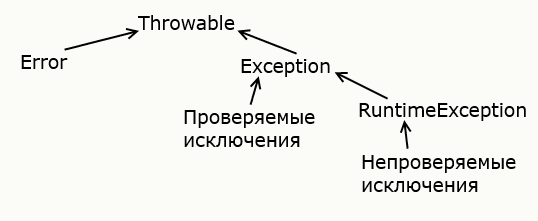
\includegraphics[width=0.8\linewidth]{pic23-1.png}
\label{fig:mpr}
\end{figure}

\section{Пользовательские классы исключений}

Иногда требуется создать свои собственные классы исключений со своей логикой. Для создания своего класса исключений надо унаследовать его от класса \verb|Exception|:

\begin{lstlisting}
class MyExceptionClass extends Exception
{

}
\end{lstlisting}

Данный класс теперь можно использовать в качестве класса исключения в необходимых случаях; кроме того, он может использовать все наследуемые методы класса \verb|Throwable| (например, \verb|getMessage()|, возвращающий описание исключения):

\begin{lstlisting}
public class TrainException {
  public static void main(String[] args) {
    MyExceptionClass mc = new MyExceptionClass();
    String str = mc.getMessage();
    System.out.println("str = " + str);
    // str = null
  }
}
\end{lstlisting}

При этом листинге выведется \verb|str = null|, т.к. сам по себе класс не возвращает сообщения, генерируемого при перехвате объекта исключения.

\section{Генерация исключений}

Как уже упоминалось ранее, ключевое слово \verb|throw| искользуется для принудительной генерации исключений в случае необходимости. Покажем пример:

\begin{lstlisting}
    ...
try {
    // ...
    throw new ThrowableClass(parameters);
}
catch (ThrowableClass e) {
    // ...
}
...
\end{lstlisting}

Внутри блока кода \verb|try| мы вызываем ключевое слово \verb|throw|, а вместе с ним также и объект класса \verb|ThrowableClass| с параметрами (если таковые есть). При этом код внутри изначального блока автоматически прерывается, и происходит переход в блок \verb|catch|, поскольку тип блока соответствует типу выброшенного исключения.

\end{document}